% Options for packages loaded elsewhere
\PassOptionsToPackage{unicode}{hyperref}
\PassOptionsToPackage{hyphens}{url}
\PassOptionsToPackage{dvipsnames,svgnames,x11names}{xcolor}
%
\documentclass[
  letterpaper,
  DIV=11,
  numbers=noendperiod]{scrreprt}

\usepackage{amsmath,amssymb}
\usepackage{lmodern}
\usepackage{iftex}
\ifPDFTeX
  \usepackage[T1]{fontenc}
  \usepackage[utf8]{inputenc}
  \usepackage{textcomp} % provide euro and other symbols
\else % if luatex or xetex
  \usepackage{unicode-math}
  \defaultfontfeatures{Scale=MatchLowercase}
  \defaultfontfeatures[\rmfamily]{Ligatures=TeX,Scale=1}
\fi
% Use upquote if available, for straight quotes in verbatim environments
\IfFileExists{upquote.sty}{\usepackage{upquote}}{}
\IfFileExists{microtype.sty}{% use microtype if available
  \usepackage[]{microtype}
  \UseMicrotypeSet[protrusion]{basicmath} % disable protrusion for tt fonts
}{}
\makeatletter
\@ifundefined{KOMAClassName}{% if non-KOMA class
  \IfFileExists{parskip.sty}{%
    \usepackage{parskip}
  }{% else
    \setlength{\parindent}{0pt}
    \setlength{\parskip}{6pt plus 2pt minus 1pt}}
}{% if KOMA class
  \KOMAoptions{parskip=half}}
\makeatother
\usepackage{xcolor}
\setlength{\emergencystretch}{3em} % prevent overfull lines
\setcounter{secnumdepth}{5}
% Make \paragraph and \subparagraph free-standing
\ifx\paragraph\undefined\else
  \let\oldparagraph\paragraph
  \renewcommand{\paragraph}[1]{\oldparagraph{#1}\mbox{}}
\fi
\ifx\subparagraph\undefined\else
  \let\oldsubparagraph\subparagraph
  \renewcommand{\subparagraph}[1]{\oldsubparagraph{#1}\mbox{}}
\fi


\providecommand{\tightlist}{%
  \setlength{\itemsep}{0pt}\setlength{\parskip}{0pt}}\usepackage{longtable,booktabs,array}
\usepackage{calc} % for calculating minipage widths
% Correct order of tables after \paragraph or \subparagraph
\usepackage{etoolbox}
\makeatletter
\patchcmd\longtable{\par}{\if@noskipsec\mbox{}\fi\par}{}{}
\makeatother
% Allow footnotes in longtable head/foot
\IfFileExists{footnotehyper.sty}{\usepackage{footnotehyper}}{\usepackage{footnote}}
\makesavenoteenv{longtable}
\usepackage{graphicx}
\makeatletter
\def\maxwidth{\ifdim\Gin@nat@width>\linewidth\linewidth\else\Gin@nat@width\fi}
\def\maxheight{\ifdim\Gin@nat@height>\textheight\textheight\else\Gin@nat@height\fi}
\makeatother
% Scale images if necessary, so that they will not overflow the page
% margins by default, and it is still possible to overwrite the defaults
% using explicit options in \includegraphics[width, height, ...]{}
\setkeys{Gin}{width=\maxwidth,height=\maxheight,keepaspectratio}
% Set default figure placement to htbp
\makeatletter
\def\fps@figure{htbp}
\makeatother

\KOMAoption{captions}{tableheading}
\makeatletter
\@ifpackageloaded{tcolorbox}{}{\usepackage[many]{tcolorbox}}
\@ifpackageloaded{fontawesome5}{}{\usepackage{fontawesome5}}
\definecolor{quarto-callout-color}{HTML}{909090}
\definecolor{quarto-callout-note-color}{HTML}{0758E5}
\definecolor{quarto-callout-important-color}{HTML}{CC1914}
\definecolor{quarto-callout-warning-color}{HTML}{EB9113}
\definecolor{quarto-callout-tip-color}{HTML}{00A047}
\definecolor{quarto-callout-caution-color}{HTML}{FC5300}
\definecolor{quarto-callout-color-frame}{HTML}{acacac}
\definecolor{quarto-callout-note-color-frame}{HTML}{4582ec}
\definecolor{quarto-callout-important-color-frame}{HTML}{d9534f}
\definecolor{quarto-callout-warning-color-frame}{HTML}{f0ad4e}
\definecolor{quarto-callout-tip-color-frame}{HTML}{02b875}
\definecolor{quarto-callout-caution-color-frame}{HTML}{fd7e14}
\makeatother
\makeatletter
\makeatother
\makeatletter
\@ifpackageloaded{bookmark}{}{\usepackage{bookmark}}
\makeatother
\makeatletter
\@ifpackageloaded{caption}{}{\usepackage{caption}}
\AtBeginDocument{%
\ifdefined\contentsname
  \renewcommand*\contentsname{Table of contents}
\else
  \newcommand\contentsname{Table of contents}
\fi
\ifdefined\listfigurename
  \renewcommand*\listfigurename{List of Figures}
\else
  \newcommand\listfigurename{List of Figures}
\fi
\ifdefined\listtablename
  \renewcommand*\listtablename{List of Tables}
\else
  \newcommand\listtablename{List of Tables}
\fi
\ifdefined\figurename
  \renewcommand*\figurename{Figure}
\else
  \newcommand\figurename{Figure}
\fi
\ifdefined\tablename
  \renewcommand*\tablename{Table}
\else
  \newcommand\tablename{Table}
\fi
}
\@ifpackageloaded{float}{}{\usepackage{float}}
\floatstyle{ruled}
\@ifundefined{c@chapter}{\newfloat{codelisting}{h}{lop}}{\newfloat{codelisting}{h}{lop}[chapter]}
\floatname{codelisting}{Listing}
\newcommand*\listoflistings{\listof{codelisting}{List of Listings}}
\makeatother
\makeatletter
\@ifpackageloaded{caption}{}{\usepackage{caption}}
\@ifpackageloaded{subcaption}{}{\usepackage{subcaption}}
\makeatother
\makeatletter
\@ifpackageloaded{tcolorbox}{}{\usepackage[many]{tcolorbox}}
\makeatother
\makeatletter
\@ifundefined{shadecolor}{\definecolor{shadecolor}{rgb}{.97, .97, .97}}
\makeatother
\makeatletter
\makeatother
\ifLuaTeX
  \usepackage{selnolig}  % disable illegal ligatures
\fi
\IfFileExists{bookmark.sty}{\usepackage{bookmark}}{\usepackage{hyperref}}
\IfFileExists{xurl.sty}{\usepackage{xurl}}{} % add URL line breaks if available
\urlstyle{same} % disable monospaced font for URLs
\hypersetup{
  pdftitle={Research methods in Cognitive Neuroscience},
  pdfauthor={Carlos González},
  colorlinks=true,
  linkcolor={blue},
  filecolor={Maroon},
  citecolor={Blue},
  urlcolor={Blue},
  pdfcreator={LaTeX via pandoc}}

\title{Research methods in Cognitive Neuroscience}
\author{\href{https://gonzalezgarcia.github.io/}{Carlos González}}
\date{}

\begin{document}
\maketitle
\ifdefined\Shaded\renewenvironment{Shaded}{\begin{tcolorbox}[borderline west={3pt}{0pt}{shadecolor}, enhanced, sharp corners, frame hidden, interior hidden, breakable, boxrule=0pt]}{\end{tcolorbox}}\fi

\renewcommand*\contentsname{Table of contents}
{
\hypersetup{linkcolor=}
\setcounter{tocdepth}{2}
\tableofcontents
}
\bookmarksetup{startatroot}

\hypertarget{welcome}{%
\chapter*{Welcome}\label{welcome}}
\addcontentsline{toc}{chapter}{Welcome}

\markboth{Welcome}{Welcome}

\begin{figure}

{\centering 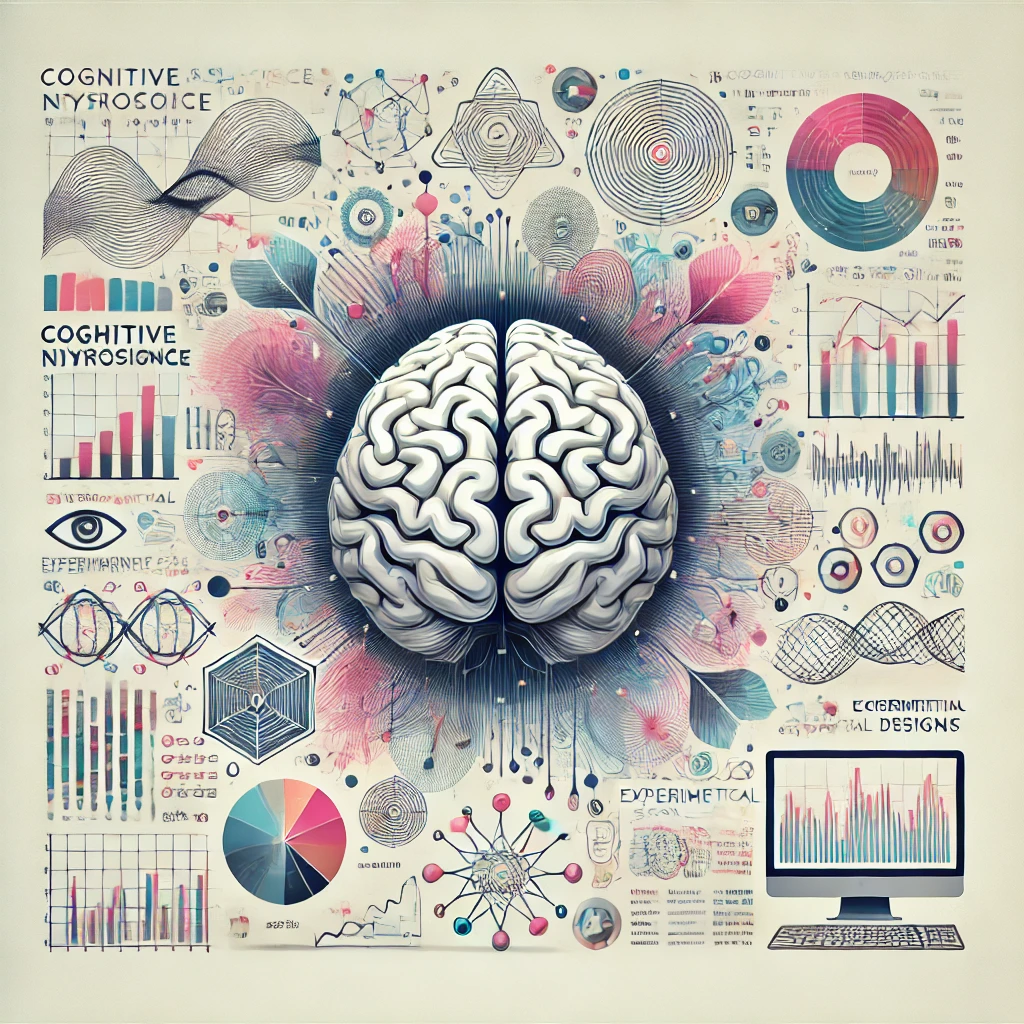
\includegraphics[width=5.20833in,height=\textheight]{chatgpt.png}

}

\caption{AI algorithm hallucinates what this course is about}

\end{figure}

This text is aimed to serve as your guide for the first half of the
course ``Methodology in Cognitive Neuroscience: Basic and Applied
Research'' in the Master's Program in Cognitive and Behavioral
Neuroscience at the University of Granada.

In this section, we will explore the foundations of experimental
research in cognitive neuroscience and develop practical skills in
experiment programming. We'll begin by introducing key concepts in
research methods and experimental thinking, providing you with a solid
theoretical foundation. Then, we'll dive into hands-on training using
\href{https://pstnet.com/products/e-prime/}{\textbf{E-Prime}} and
\href{https://osdoc.cogsci.nl/}{\textbf{OpenSesame}}, two powerful
pieces of software for creating psychology experiments.

By the end of this module, you will be able to:

\begin{itemize}
\tightlist
\item
  Understand and apply principles of experimental design in cognitive
  neuroscience
\item
  Think critically about research methodology and experimental control
\item
  Design and program your own experiments using E-Prime and OpenSesame
\item
  Troubleshoot common issues in experiment programming
\end{itemize}

This guide is designed to be both theoretical and practical. Most of the
chapters include conceptual discussions followed by hands-on exercises
to help you apply what you've learned. Remember, mastering these skills
requires practice, creativity, and persistence!

\begin{tcolorbox}[enhanced jigsaw, opacitybacktitle=0.6, arc=.35mm, colbacktitle=quarto-callout-tip-color!10!white, bottomrule=.15mm, titlerule=0mm, coltitle=black, title=\textcolor{quarto-callout-tip-color}{\faLightbulb}\hspace{0.5em}{Relevant links}, toprule=.15mm, left=2mm, colback=white, rightrule=.15mm, bottomtitle=1mm, colframe=quarto-callout-tip-color-frame, opacityback=0, toptitle=1mm, breakable, leftrule=.75mm]

\href{https://masteres.ugr.es/neurocg/docencia/plan-estudios/guia-docente/M30/56/2/27}{Course
guide}

\end{tcolorbox}

\begin{tcolorbox}[enhanced jigsaw, opacitybacktitle=0.6, arc=.35mm, colbacktitle=quarto-callout-warning-color!10!white, bottomrule=.15mm, titlerule=0mm, coltitle=black, title=\textcolor{quarto-callout-warning-color}{\faExclamationTriangle}\hspace{0.5em}{Disclaimer}, toprule=.15mm, left=2mm, colback=white, rightrule=.15mm, bottomtitle=1mm, colframe=quarto-callout-warning-color-frame, opacityback=0, toptitle=1mm, breakable, leftrule=.75mm]

This material has been elaborated for the use of the Cognitive
Neuroscience master students of the Universidad de Granada, years
2023-25.

The resources listed here are Open Educational Resources (OER) that are
free to use, share, copy, and edit, with attribution, following the
terms of the specified license.

Please contact \href{https://ugr.es/~cgonzalez}{Carlos González} for any
inquiry.

\end{tcolorbox}

\bookmarksetup{startatroot}

\hypertarget{syllabus}{%
\chapter{Syllabus}\label{syllabus}}

\hypertarget{required-software}{%
\section{Required Software}\label{required-software}}

Check PRADO for instructions on how to install \textbf{E-Prime}.

\textbf{OpenSesame} (download latest version from
\href{https://osdoc.cogsci.nl/4.0/download/}{here}).

It should run in any more or less recent computer. If you have any issue
installing it, please let me know as soon as possible!

\hypertarget{resources-and-recommended-readings}{%
\section{Resources and recommended
readings}\label{resources-and-recommended-readings}}

\begin{tcolorbox}[enhanced jigsaw, opacitybacktitle=0.6, arc=.35mm, colbacktitle=quarto-callout-note-color!10!white, bottomrule=.15mm, titlerule=0mm, coltitle=black, title=\textcolor{quarto-callout-note-color}{\faInfo}\hspace{0.5em}{Note}, toprule=.15mm, left=2mm, colback=white, rightrule=.15mm, bottomtitle=1mm, colframe=quarto-callout-note-color-frame, opacityback=0, toptitle=1mm, breakable, leftrule=.75mm]

Note: these are just extra readings in case you want to learn more. They
are encouraged but not required to follow or pass the course.

\end{tcolorbox}

\begin{itemize}
\tightlist
\item
  Barbosa, J., Stein, H., Zorowitz, S., Niv, Y., Summerfield, C.,
  Soto-Faraco, S., \& Hyafil, A. (2023). A practical guide for studying
  human behavior in the lab. Behavior Research Methods, 55(1), 58-76.
\item
  Frank, M. C., Braginsky, M., Cachia, J., Coles, N.A., Hardwicke, T.E.,
  Hawkins, R.E., Mathur, M.B., and Williams, R. 2024. Experimentology:
  An Open Science Approach to Experimental Psychology Methods. MIT
  Press. https://doi.org/10.7551/mitpress/14810.001.0001.
\item
  Mathôt, S., Schreij, D., \& Theeuwes, J. (2012). OpenSesame: An
  open-source, graphical experiment builder for the social sciences.
  Behavior Research Methods, 44, 314-324.
\item
  Myers, J. L., Well, A. D., \& Lorch Jr, R. F. (2013). Research design
  and statistical analysis. Routledge.
\end{itemize}

\hypertarget{assessment}{%
\section{Assessment}\label{assessment}}

This course is divided in two parts:

\begin{enumerate}
\def\labelenumi{\arabic{enumi})}
\item
  Programming of experiments (50\% of the final grade)
\item
  Statistical analyses (50\% of the final grade)
\end{enumerate}

\begin{tcolorbox}[enhanced jigsaw, opacitybacktitle=0.6, arc=.35mm, colbacktitle=quarto-callout-warning-color!10!white, bottomrule=.15mm, titlerule=0mm, coltitle=black, title=\textcolor{quarto-callout-warning-color}{\faExclamationTriangle}\hspace{0.5em}{Important!}, toprule=.15mm, left=2mm, colback=white, rightrule=.15mm, bottomtitle=1mm, colframe=quarto-callout-warning-color-frame, opacityback=0, toptitle=1mm, breakable, leftrule=.75mm]

A minimum of 25\% in each phase is required to pass the course.

\end{tcolorbox}

In my part of the course (\emph{Part 1}), your final grade will depend
on:

\begin{longtable}[]{@{}lc@{}}
\toprule()
Activity & Contribution to final grade \\
\midrule()
\endhead
Participation and in-class assignments & 30\% \\
Individual programming assignments & 30\% \\
Final project & 40\% \\
\bottomrule()
\end{longtable}

\hypertarget{course-policies}{%
\section{Course Policies}\label{course-policies}}

\hypertarget{attendance-and-participation}{%
\subsection{Attendance and
Participation}\label{attendance-and-participation}}

Attendance is strongly encouraged for this course due to its eminently
practical nature. Please note:

\begin{itemize}
\tightlist
\item
  Many in-class activities and hands-on exercises might not be easily
  replicated outside of class.
\item
  Regular attendance will significantly enhance your learning experience
  and ability to complete assignments successfully.
\item
  If you must miss a class, it is your responsibility to catch up on
  missed material and assignments.
\item
  Consistent participation in class discussions and activities will
  positively impact your learning and final grade.
\end{itemize}

\hypertarget{late-work-and-extensions}{%
\subsection{Late Work and Extensions}\label{late-work-and-extensions}}

\begin{itemize}
\tightlist
\item
  Assignments are due on the dates specified in the course schedule.
\item
  Late submissions will incur a 20\% penalty
\item
  If you anticipate difficulty meeting a deadline, please contact me as
  soon as possible to discuss potential extensions.
\item
  Extensions may be granted for documented emergencies or extenuating
  circumstances at the instructor's discretion.
\end{itemize}

\hypertarget{academic-integrity}{%
\subsection{Academic Integrity}\label{academic-integrity}}

\begin{itemize}
\tightlist
\item
  All work submitted must be your own.
\item
  When using external sources (including generative AI tools), proper
  citation is required.
\item
  Collaboration on assignments is encouraged, but each student must
  submit their own original work.
\end{itemize}

\hypertarget{communication}{%
\subsection{Communication}\label{communication}}

\begin{itemize}
\tightlist
\item
  Email (\texttt{cgonzalez\ at\ ugr\ dot\ es}) is the primary mode of
  communication outside of class.
\item
  You can also use PRADO if you prefer.
\end{itemize}

\hypertarget{office-hours}{%
\section{Office Hours}\label{office-hours}}

Mondays from 8:30 to 11, but feel free to send me an email anytime or
just ask me after class.

\bookmarksetup{startatroot}

\hypertarget{session-0}{%
\chapter{Session 0}\label{session-0}}

\hypertarget{from-research-questions-to-data}{%
\section{From Research Questions to
Data}\label{from-research-questions-to-data}}

The essence of cognitive neuroscience experiments is to examine
relationships between manipulations (independent variables) and their
effects on measurable outcomes (dependent variables). Remember there are
various experimental designs, such as:

\begin{itemize}
\tightlist
\item
  \textbf{Between-participants design}: Each participant experiences
  only one level of a factor.
\item
  \textbf{Within-participants design}: Participants experience multiple
  levels of a factor, allowing for within-subject comparisons.
\item
  \textbf{Mixed designs}: Combining elements of both between- and
  within-participant designs.
\end{itemize}

There are also techniques like \textbf{counterbalancing} to mitigate
order effects and ensure reliable, replicable results.

\hypertarget{tools-for-experimental-design}{%
\section{Tools for Experimental
Design}\label{tools-for-experimental-design}}

During the programming phase, you'll become familiar with two key
software tools:

\hypertarget{e-prime}{%
\subsection{E-Prime}\label{e-prime}}

\begin{itemize}
\tightlist
\item
  Widely used at CIMCYC
\item
  Great for users with little coding experience
\item
  Only available on Windows (License required; check PRADO)
\end{itemize}

\hypertarget{opensesame}{%
\subsection{OpenSesame}\label{opensesame}}

\begin{itemize}
\tightlist
\item
  Python-based and open source
\item
  Cross-platform and free
\item
  Requires basic coding knowledge, but has a large online community
\end{itemize}

If you need help accessing these tools or have a non-Windows computer,
feel free to reach out!

\begin{tcolorbox}[enhanced jigsaw, opacitybacktitle=0.6, arc=.35mm, colbacktitle=quarto-callout-tip-color!10!white, bottomrule=.15mm, titlerule=0mm, coltitle=black, title=\textcolor{quarto-callout-tip-color}{\faLightbulb}\hspace{0.5em}{Relevant readings}, toprule=.15mm, left=2mm, colback=white, rightrule=.15mm, bottomtitle=1mm, colframe=quarto-callout-tip-color-frame, opacityback=0, toptitle=1mm, breakable, leftrule=.75mm]

For more reading, check out the following resources:

\begin{itemize}
\tightlist
\item
  \href{https://granatensis.ugr.es/discovery/fulldisplay?docid=alma991014333689904990\&context=L\&vid=34CBUA_UGR:VU1}{Myers,
  Well, \& Lorch (2013). Research Design and Statistical Analysis}
\item
  \href{https://experimentology.io/}{Experimentology}
\item
  \href{https://jmourabarbosa.github.io/files/Barbosa_2022_BRM.pdf}{Barbosa
  (2022)}
\end{itemize}

\end{tcolorbox}

Below, you can find the slides from this session:



\end{document}
